\chapter{The wildfire-habitat connectivity dilemma: a graph theoretical approach to landscape management}

\begin{center}
\textbf{Abstract}\par
    \vspace*{.2cm}
    \noindent
    \begin{minipage}{0.9\textwidth}
	\singlespacing
\textbf{Background:} Fuel treatment operations help to mitigate the spread and severity of wildfires in numerous ecosystems. As they aim at fragmenting the fire landscape, they also fragment wildlife habitat. This poses a dilemma for land managers, in the form of a trade-off between lowering wildfire patch connectivity and maintaining wildlife habitat connectivity. Previous studies have investigated the spatial allocation of fuel treatments over time, mostly without specific care devoted to biodiversity, in a variety of case studies. However, they lack generality and an interpretative framework. We use dynamic programming and graph theory on every possible theoretical landscape configuration to gain a general understanding of the allocation of treatments over space and time and the corresponding landscape properties with various habitat connectivity targets. 
 
\textbf{Results:} Our results show that all initial landscapes converge to steady-state landscape cycles. Moreover, we show that there exist optimal trajectories that significantly reduce wildfire risk while safeguarding habitat connectivity. As the policy budget increases, more risk reduction is achieved, albeit with a decreasing marginal efficiency, and more steady-state cycles emerge. As habitat targets increase, increasing the budget is of no effect, and risk increases, while the number of steady-state cycles decreases. Landscapes are less risky, more fragmented, and diverse when the budget is large and biodiversity targets are low, while they are more compact and less diverse when the opposite is true. Treatment allocation follows graph centrality measures, and central cells are treated first. When the budget increases, fewer central cells (i.e. edge \textbf{patches}) are treated as well. When biodiversity targets increase, central cells are no longer treated as they decrease habitat connectivity. Treatment is reshuffled to the edges of the landscape.


 \textbf{Conclusion:} Computational experiments generalize existing results. Using graph theory, general insights can be gained, and help managers faced with multiple objectives in forested landscapes. From a policy perspective, in the face of climate change, increasing treatment budgets should be a priority to avoid increasing damages. A key guideline is treating a variety of seral stages to create landscape diversity, mitigate risk and guarantee the connectivity of wildlife habitat. 
\\
\textbf{Keywords : }Fuel treatment, connectivity, wildfire risk, wildlife habitat, spatial optimization, graph theory
\end{minipage}
\end{center}

\vfill
\newpage
\section*{To do}

\subsection*{Analysis}
\begin{itemize}
\item Run sample analysis for successive optimization
\item Compare outcomes
\begin{itemize}
\item Compare FPPs
\item Compare locations of treatments : centrality, degree etc
\item Compare landscapes characteristics
\end{itemize}
\item Need to think of the 5 period optimization v. the 3 age structure. 
\end{itemize}
\subsection*{Purpose of the paper}
\begin{itemize}
\item Launch all of the analysis : impossible for dynamic optimization
\item We do a subsample of 300 landscapes for real dynamic optimization: can generalize the findings 
\item We compare and find the general rules in a probabilistic sense
\item Then we find globally applicable rules of treatment allocation
\item Then we test them on large scale landscapes (100x100) and we test with different strategies: 
\begin{itemize}
\item Treat only old cells
\item Treat only young cells
\item Treat central cells
\item Treat a lot now, and less in the future (e.g. shift the budget towards today)
\end{itemize}
\end{itemize}

\subsection*{Rewriting}
\begin{itemize}
\item Justify why this is an economics problem
\begin{itemize}
\item We look at the social planner solution, and not the decentralized problem, because of the spatial, stochastic externality : space creates an interdependence and stochastic nature tends to cause underprotection.
\item Public ownership of land
\item Budget constraint
\item Scale 
\end{itemize}
\item Need to reinforce the widlfire risk/biodiversity relationship : 
\begin{itemize}
\item Redo literature review to link the two
\item Show clear examples with graphs
\end{itemize}
\item Need to reinforce our contribution in terms of what the problem is, and how our analysis is innovative : 
\begin{itemize}
\item Dynamic MILP : we do 5 periods : how do they relate to real life and how can we justify it? 
\item The former point implies the curse of dimensionality
\item In terms of graphs : we do not really do it in terms of coding, but we do it
\item NP hardness etc
\item Compare with existing literature, including the ones from the reviewers : network flow, or corridor : this is a single species view, or a hotspot to hotspot view, we do offer a view for multi level, multi functional biological diversity, not just the hotspots. THe question of the scale of movement of considered species is of course key. We adopt a broader view?
\item Need to write the model in a better way : fuck \textit{Fire Ecology}. 
\end{itemize}

\end{itemize}

\clearpage

\onehalfspacing
%%% Manuscript
\section{Introduction}
% Motivation : why should we care about wildfires? 
\hspace*{1.5em}Hazardous and intense wildfires destroy forest cover\footnote{From 2001 to 2023, forest loss attributed to wildfires amounted to 138 million hectares (roughly 33\% of the surface of the European Union) \citep{tyukavina_global_2022}}, threaten forest resilience and can cause ecosystem shifts, ranging from changes in forest structure to changes towards non-forest ecosystems \citep{coop_wildfire-driven_2020}. 
Additionally, intense wildfires cause human damages, in the form of direct asset losses: in 2018, wildfires in California have caused \$ 27 billion \citep{wang_economic_2021}. Indirect costs are also of concern, especially related to wildfire smoke : increases in PM 2.5 concentrations have important health impacts \citep{burke_wildfire_2023, heft-neal_behavior_2023}, smoke directly affects recreation values in the US, amounting to \$USD 2.3 billion in welfare losses \citep{Gellman}. Aside from directly measurable costs, wildfires also cause dramatic impacts on biodiversity across taxa \citep{Wintle2020}, through direct population losses and durable habitat disruption \citep{Ayars2023}.
%
\\
\hspace*{1.5em}In a business as usual scenario in terms of forest management, wildland-urban interface expansion and climate change, these direct and indirect costs and damages to both humans and non-humans are expected to increase drastically.
%
\\
Decades of wildfire suppression have created a ``wildfire deficit'', which increases the probability, extent and severity of wildfires in the western United States \citep{kreider_fire_2024}. European forests are not adapted to climate change induced wildfire risks \citep{Khabarov2014ForestFA}, in terms of species composition and use of fuel management operations. Mechanical thinning, prescribed burns, and sometimes, logging, have been leveraged to decrease the fuel load in risky areas and theoretically decrease the probability and severity of burns upon wildfire occurence\footnote{The efficiency of these measures depends on environmental and terrain variables. For example, prescribed burns are efficient every 1-4 years in reducing risk and severity only in the case of non-extreme weather conditions, and when the terrain ruggedness is limited \citep{bradstock_1998}}. In numerous regions, such as conifer forests in California \citep{Vaillant2009, Kalies2016, low_shaded_2023}, eucalypt forests in South Western Australia \citep{burrows2013, boer_long-term_2009, Florec2020}, southern Europe \citep{Fernandes2013}, evidence shows that fuel treatments, can mitigate wildfire intensity and spread. Land management agencies have historically implemented these policies in Australia \citep{burrows2013}, Europe, and the United States (and are projected to ramp up, for example under the Infrastructure Investment and Jobs Act of 2021 in the US). While potentially useful, the use of these treatments is still hindered by numerous obstacles \citep{miller_barriers_2020} and remains insufficient \textbf{ref}\footnote{However, recent bills have been passed in the US (Infrastructure Investment and Jobs Act of 2021) and California to ramp up the use of prescribed burns - such as \href{https://wildfiretaskforce.org/about/expenditure-plan/}{the bugdget act of 2022}, committing \$2.8 billion to the Governor’s Wildfire and Forest Resilience Action Plan - and limiting liabilities in the case of wildfire escape (see \href{https://openstates.org/ca/bills/20212022/SB332/}{California Senate Bill SB-332}) on private land.}. 
Additionally, the extension of wildland-urban interfaces (WUI) increases the extent of potential damages as well as ignition probabilities \citep{radeloff_rapid_2018}.
\\
As global warming affects water supply and fuel moisture \citep{jolly_climate-induced_2015, Abatzoglou, ruffault_extreme_2018}, it is projected to increase the frequency, severity, and magnitude of wildfires \citep{Dupuy2019ClimateCI, wasserman_climate_2023}. Recent wildfire events in California (since 2018), in Australia (2019-2020), and in Europe (France, Portugal, Greece in 2022) have epitomized these trends. 
%
Moreover, wildfires and climate change are endogeneously linked in a positive feedback loop : large wildfires are of importance in the face of climate change; as they release large amounts of greenhouse gases ($1.7GtC$ per year on average between 2003 and 2022) and reduce the extent of terrestrial carbon sinks \citep{zheng_record-high_2023, friedlingstein_2023}. \\
\hspace*{1.5em}In the face of a growing threat to human assets and biological diversity, increasing the efficiency of fuel treatments to manage multiple objectives is paramount. A decision framework that accounts for wildfire processes and biological diversity drivers is paramount to deliver policy recommendations that simultaneously achieve widlfire damage reduction and protect biological diversity \citep{driscoll_resolving_2010}. Among the decision levers, the extent and location of treatments are key variables. 
%
\\
By changing the structure of the landscape, fuel management operations may reduce the risk and associated damages of wildfires. Treatments achieve larger risk reduction when located close to the values at risk instead of being dispersed across the landscape \citep{ager_modeling_2007, Williams2017,Florec2020}. However, they also affect the structure of biodiversity habitat, notably, its structural connectivity \citep{Taylor93}. Maintaining habitat connectivity, through wildlife corridors, landscape links, and ecoducts \citep{Turner2005, Turner2011}, is instrumental in mitigating the biodiversity crisis. Species richness and diversity are intimately linked to landscape connectivity \citep{Olds2012, tian_assessing_2017, velazquez_structural_2019} and are necessary to maintain ecosystems in the future. Fragmentation, conditional on habitat surface being constant, may enhance biodiversity \citep{tischendorf_usage_2000, hu_effects_2012, may_geometry_2019}. However, it is often accompanied with habitat loss, detrimental to biodiversity \citep{fahrig_effects_2003}. The use of fuel management operations alters the structure of the landscape e.g. both habitat and matrix\footnote{e.g. land use or cover, or environmental conditions that differ from eitehr species' habitat or reference natural conditions \citep{fletcher_prominent_2024}}, in terms of temporal and spatial variation in landscape configuration and composition. As habitat is altered, so is the surrounding matrix, which can impede species movement \citep{eycott_meta-analysis_2012, kuefler_conflicting_2010} and alter evolution and selective regimes \citep{cheptou_adaptation_2017}.\\
The impact of fuel treatments on biodiversity remains a debated topic. 
Evidence suggests that maintaining a variety of vegetation types and ages on a patchy landscape maintains a 'fire mosaic' \citep{Sitters2015} (e.g. landscape level variations in habitat types that provide habitat to an ecological community) or that fuel treatment can be beneficial to wildlife \citep{saab_short-term_2022, loeb_bats_2021} and even restore local populations \citep{Templeton2011}. On the other hand, treating at too high a frequency may be detrimental to biodiversity \citep{bradshaw2018}, as vegetation with extensive juvenile period may disappear, and fauna that rely on them as well\footnote{For example, in Australia, species such as \textit{Banksia baueri}, \textit{B. nutans} and B. \textit{baxteri} would disappear, threatening tammar wallabies, quokas and honey possums \citep{bradshaw2018}}, or high frequency treatment favors the invasion of fire tolerant, fire-enhanced weed species \citep{vanWilgen_fire_2013}. 
%
\\
Hence, fragmenting the wildfire risk poses significant threats to biodiversity in forest landscapes. Nonetheless, there may exist a range of spatial allocation patterns that take into account the location of protected species and can reduce threats to both assets and biodiversity \citep{ager_modeling_2007, king_relative_2008, rachmawati_fuel_2018}. 
\\
\hspace*{1.5em}Eventually, wildfire risk and potential damages pose a significant challenge in terms of policy-making. As wildfire risks and potential damages are spatially heterogeneous, and as wildfires spread, they create a large spatial externality. Indeed, individual risk reduction is hampered by the influence of neighbors on individual risk, which results in the under provision of risk reduction \citep{SHAFRAN2008488, costello_private_2007}. Additionally, in a risky (e.g. stochastic) context, risk aversion may bolster this phenomenon when financial insurance is limited \citep{ehrlich_market_1972}\footnote{This is particularly the case in California, where repeated fire episodes have pushed insurers to \href{https://calmatters.org/economy/2024/05/california-insurance-mitigation/}{spike contract premiums}, or \href{https://www.nbclosangeles.com/news/california-wildfires/state-farm-california-los-angeles-homeowners-insurance-policy/3383583/}{to not renew contracts}- non renewal rates went from 11\% in 2018 to 13\% in 2021}. Finally, the magnitude of potential damages \citep{costello_private_2017} as well as the large information requirements for efficient fuel treatment planning warrant a collective approach.
\\
\hspace*{1.5em}In this context, we study the spatial patterns of treatment allocation that diminish potential damages from wildfires in where fire spread is governed by patch connectivity, while safeguarding biodiversity habitat connectivity, from a central decision maker perspective.  
\\
\hspace*{1.5em}A substantial literature has applied optimization techniques to tackle the spatial allocation of fuel treatments. Analytical \citep{finney_design_2001}, simulation-based \citep{finney_computational_2007, rytwinski_simulation-optimization_2010} or mixed-integer programming techniques \citep{wei_optimization_2008} have solved the allocation of treatments in a static framework. Given the dynamic nature of fuel growth, studies based on mixed-integer dynamic programming \citep{wei_optimization_2008, minas_spatial_2014, rachmawati_model_2015, rachmawati_optimisation_2016} have studied the temporal and spatial allocation of fuel treatments on real and simulated landscapes. While they solve the spatial treatment allocation problem in forests, these articles fail to acknowledge the multiple uses and objectives land planners have to consider, such as habitat conservation. Several articles have devoted their attention to the spatial allocation of treatments while conserving habitat, and investigated the trade-offs between risk reduction and biodiversity conservation, using spatial heuristics \citep{calkin_modeling_2005, lehmkuhl_seeing_2007} and linear programming \citep{Williams2017, rachmawati_fuel_2018}.\\
Most of the existing literature focuses on case studies and lacks a general interpretative framework to generalize its results. Graph theory offers a toolbox suited to analyze the properties of connected cells or patches of land with varying characteristics, and has extensively been applied in landscape ecology \citep{urban_landscape_2001, minor_graph-theory_2008, rayfield_multipurpose_2016}. \cite{conrad_wildlife_2012} and \cite{jafari_new_2013} use a specific graph theory algorithm - a network-flow model - to find the optimal subgraph of corridors connecting habitat areas. Their approach optimally connects patches of habitat spread across the landscape for a given species, in a reserve-network design problem fashion. Our approach adopts a more holistic perspective, as it emphasises the degree of connectedness between habitat cells, thus allowing for a multi-species and multi-scale perspective, instead of a corridor for a single species.  
\\
Recent research focusing on the allocation of fuel treatments has leveraged tools from graph theory \citep{matsypura_wildfire_2018, pais_downstream_2021}. Reconciling habitat and wildfire risk mitigation using graph theory is a recent research endeavor \citep{rachmawati_fuel_2018, yemshanov_exploring_2022} and has focused on specific case studies. 
\\\\
\hspace*{1.5em} In this article, we focus on the dynamic and spatial dimensions of the problem (thus abstracting from the stochastic components) and leverage graph theory to study the general patterns of treatment allocation emerging from a multi-objective, dynamic, and integer landscape management problem, governed by connectivity. \\
To do so, we first compare the optimal allocation of treatments using repeated static optimization and heuristic dynamic programming on a 5 period horizon on representative subsamples of small scale landscapes with an exhaustive range of habitat connectivity constraint. We show that for realistic biodiversity habitat constraint levels, the constraint imposed on the evolution of the forest results in similar structures for repeated myopic and dynamic optimization. Therefore, we analyse the treatment allocation and landscape structures emerging in the long run using repeated myopic optimization for all the possible initial landscape configurations, in a graph theoretical framework. We explicit the trade-off between risk reduction and biodiversity habitat, in the form of a production possibility frontier (PPF). We characterize the landscapes using a range of ecological indicators and find general mechanisms and guiding principles applicable to a broad class of settings, to guide decision-makers and foster new efficient multi-objective graph theory algorithms. Finally, we test our predictions from a small scale landscape to simulated realistic large scale landscapes (10,000 cells)  with varying composition and spatial autocorrelation, and compare them with different intuitive policy recommendations. 
\\
Our contributions are several. First, we provide a spatial framework to understand the trade-offs between wildfire risk reduction and biodiversity conservation. Second, we leverage the constraints imposed on a dynamic spatial system to show that repeated optimization performs relatively well compared to dynamic programming. Third, using graph theory, we derive general principles regarding the spatial characteristics of landscapes and treatments from an exhaustive set of theoretical landscapes to guide policymakers as well as future research in heuristics to reconcile conflicting land-based phenomenons.
%Eventually, we characterize the risk and biodiversity profiles consistent with a changing climate, where windows of opportunity are shorter and costs of treatment larger, and the associated spatialized treatments. 
\\
This article is structured as follows : section \ref{section:methods} explains our methods, section \ref{sec:results} explains our results, and section \ref{section:discussion} discusses our results and concludes. 

\section{Methods}
\label{section:methods}
\subsection{Model description}

%\subsection{Context}
We consider landscapes represented by a regular grid of $n\times n$ standardized area cells in period $t$ by $\mathbf{A}_t$ with a forest seral stage succession module. 
%We denote by $\mathbf{A}_t$ the matrix of standardized area cells in the theoretical landscape of dimension $n\times n$ (hereafter referred to as being of size$=n$) in period $t$. 
Each cell $a_{ijt} \in \mathbf{A}_t$ with $\{i,j\} \in \{1, ...,n\}^2$, at time $t$ is characterized by a successional stage: \textit{juvenile}, \textit{adolescent}, or \textit{mature}, which translates into 3 numerical age classes ranging from 0 to 2. 
Each transitionary seral stage has the same duration\footnote{For example, in Australia, \cite{mccoll_gausden_pathways_2019} use quasi evenly spaced age classes for heathland, tall-mixed, foothills, forby and wet vegetation types (see table 1); on the other hand, in coniferous forests in Western US (Washington and Oregon),\cite{thomas_wildlife_1979} developed a successional stage description for wildlife habitat management, \href{https://www.fs.usda.gov/Internet/FSE_DOCUMENTS/stelprdb5413728.pdf}{still used by the USDA}. 40 year transitional classes can be made grouping \textit{grass-forb, shrub-seedling and pole-sapling} together and \textit{young}. \textit{Maturity} is reached at 80 until 159 years old, where it mutates into \textit{old-growth}}, hence at each time step, it changes stage until it is in the \textit{mature} stage, where it remains (eq \ref{eq:fuel_dyn})

We use a stylized representation of the link between vegetation age, habitat, and wildfire risk (figure \ref{fig:illustration}). \\
First, we assume a cell offers suitable wildlife habitat once it is \textit{adolescent} (eq. \ref{eq:mature}). Second, a cell can turn at critical risk of wildfire during a normal hot season when its successional stage is \textit{mature} (eq. \ref{eq:high_fuel}). We assume an Olsen-type model of flammability, where age class is the main predictor of flammability \citep{Olson1963,mccarthy_theoretical_2001,mccoll_gausden_pathways_2019}. A cell remains at high risk as long as it is in the \textit{mature} age class. \\
Finally, we consider fuel treatment to be a binary decision e.g. treatment is absent or present and there is no extensive margin, hence a treatment binary variable $x_{ijt}\in\{0,1\}$ represents the treatment status in cell $a_{ij}$ a time $t$. The decision maker first observes the transition to the next successional stage, then decides upon treatment.
Treatment can happen at any successional stage : whether at an \textit{adolescent} stage, in anticipation of a cell becoming \textit{mature} and turning at \textit{high risk} in the next period, or as an immediate strategy upon becoming \textit{mature} and thus, \textit{high risk}.
Upon treatment, a cell successional stage is reset to \textit{juvenile} (eq. \ref{eq:fuel_dyn}). Figure \ref{fig:illustration} illustrates the dynamics of the model.

Given a patch $a_{ijt}$ and treatment status $x_{ijt}$ in period $t$, equation \ref{eq:fuel_dyn} summarises the successional dynamics, and equations \ref{eq:high_connectivity},\ref{eq:high_fuel} summarize the link between successional stage, habitat, and high risk: $\forall t, \forall \{i,j\} \in \{1,..., n\}^2$

%\begin{minipage}{0.45\textwidth}
   \begin{align}
a_{ijt+1} &= \max \large((a_{ijt} + 1)(1-x_{ijt}); 2 \large)
\label{eq:fuel_dyn}\\
Habitat\left(a_{ijt}\right) &= \begin{cases}
        1 &\text{ if } a_{ijt} \geq 1\\
        0 &\text{ otherwise }
    \end{cases}
\label{eq:mature}\\
Risk\left(a_{ijt}\right) &= \begin{cases}
1 &\text{ if }a_{ijt}\geq 2\\
0 &\text{ otherwise}
    \end{cases}
\label{eq:high_fuel}
\end{align}
%\end{minipage}%
\hfill
\begin{figure}
    \centering
    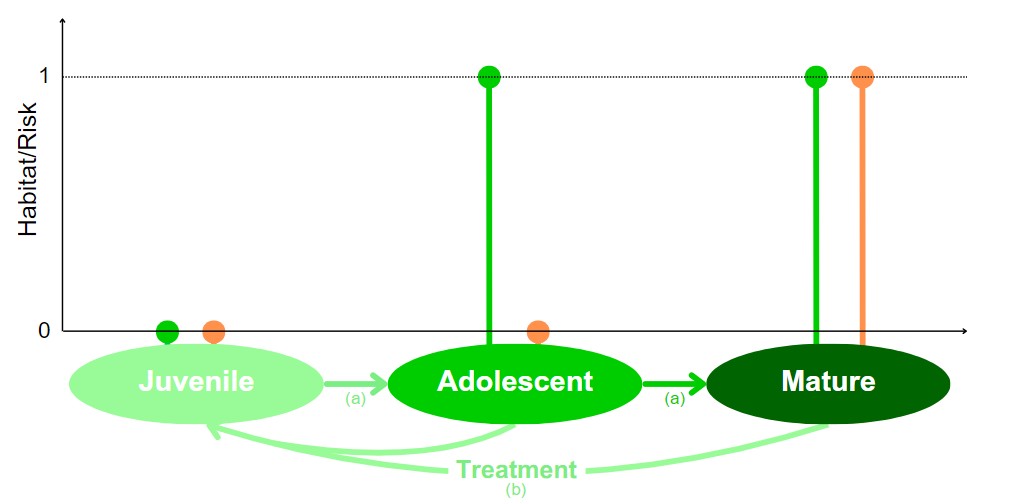
\includegraphics[width = .6\textwidth]{figures/wildland/Juvenile.png}
    \caption{Illustration of the successional stages and the link between successional stage, habitat and wildfire risk using a discretized Olson-type relationship}
    \subcaption*{At the bottom, the dynamics of the model are illustrated. First, successional stages transition (step (a)), then treatment is applied (step (b)). At the top, the link between successional stage, habitat and high risk. In green, a \textit{habitat} variables turns to $1$ when a cell is \textit{adolescent}, and in orange, a \textit{high risk} dummy turns to $1$ when a cell turns \textit{mature}} 
    \label{fig:illustration}
\end{figure}
%\end{minipage}%


%\subsection{Theoretical model}

We use a network structure to apprehend the landscapes. From the matrix $\mathbf{A}_t$, we form two graphs:  $\mathcal{B}_t = (V_{\mathcal{B}_t}, E_{\mathcal{B}_t})$, the graph of suitable habitat cells and $\mathcal{F}_t = (V_{\mathcal{F}_t}, E_{\mathcal{F}_t})$, the graph of high risk cells. First, the vertices of each graphs are the suitable habitat cells e.g $
V_{\mathcal{B}_t} = \{(i,j)$ such that $Habitat(a_{ijt})=1\}$ and the high risk cells, respectively e.g. $V_{\mathcal{F}_t} = \{(i,j)$ such that $Risk(a_{ijt})=1\}$.\\
Second, vertices are connected if they are within a Moore (or 8-cell) neighborhood of each other and share the same status. Therefore, notice that $\mathcal{F}_t\subset \mathcal{B}_t$. Figure \ref{fig:graph_overlap} illustrate the mechanism from the landscape in matrix form $\mathbf{A}_t$ with age classes ranging from 0 to 2, to graphs $\mathcal{B}_t$ and $\mathcal{F}_t$.

We use this 8-cell neighborhood for evaluating biodiversity habitat and wildfire risk within a common a spatial framework, using the same adjacency properties. 
Regarding biodiversity, we focus on general characteristics related to landscape structural connectivity rather than functional connectivity, as we are agnostic about effective species \citep{Fahrig2011}. We assume that species are able to disperse from one patch to another, and that habitat quality is uniformly distributed conditional on habitat being available.\\
We consider the wildfire risk through the lens of potential spread, influenced by fuel, wind direction and terrain. We abstract from wind patterns and terrain, to focus on fuel connectivity\footnote{Note that our framwork is amenable to prevailing wind patterns and terrain ruggedness, as the graph adjacency matrix can change from a Moore adjacency to any pattern influenced by environmental features}. Consistent with the literature (see \cite{Peterson_2009}, \cite{pais_cell2fire_2021, gonzalez-olabarria_fire_2023}), a wildfire can spread in any direction, conditional on neighbor cells with high risk. 

\begin{figure}
    \centering
    %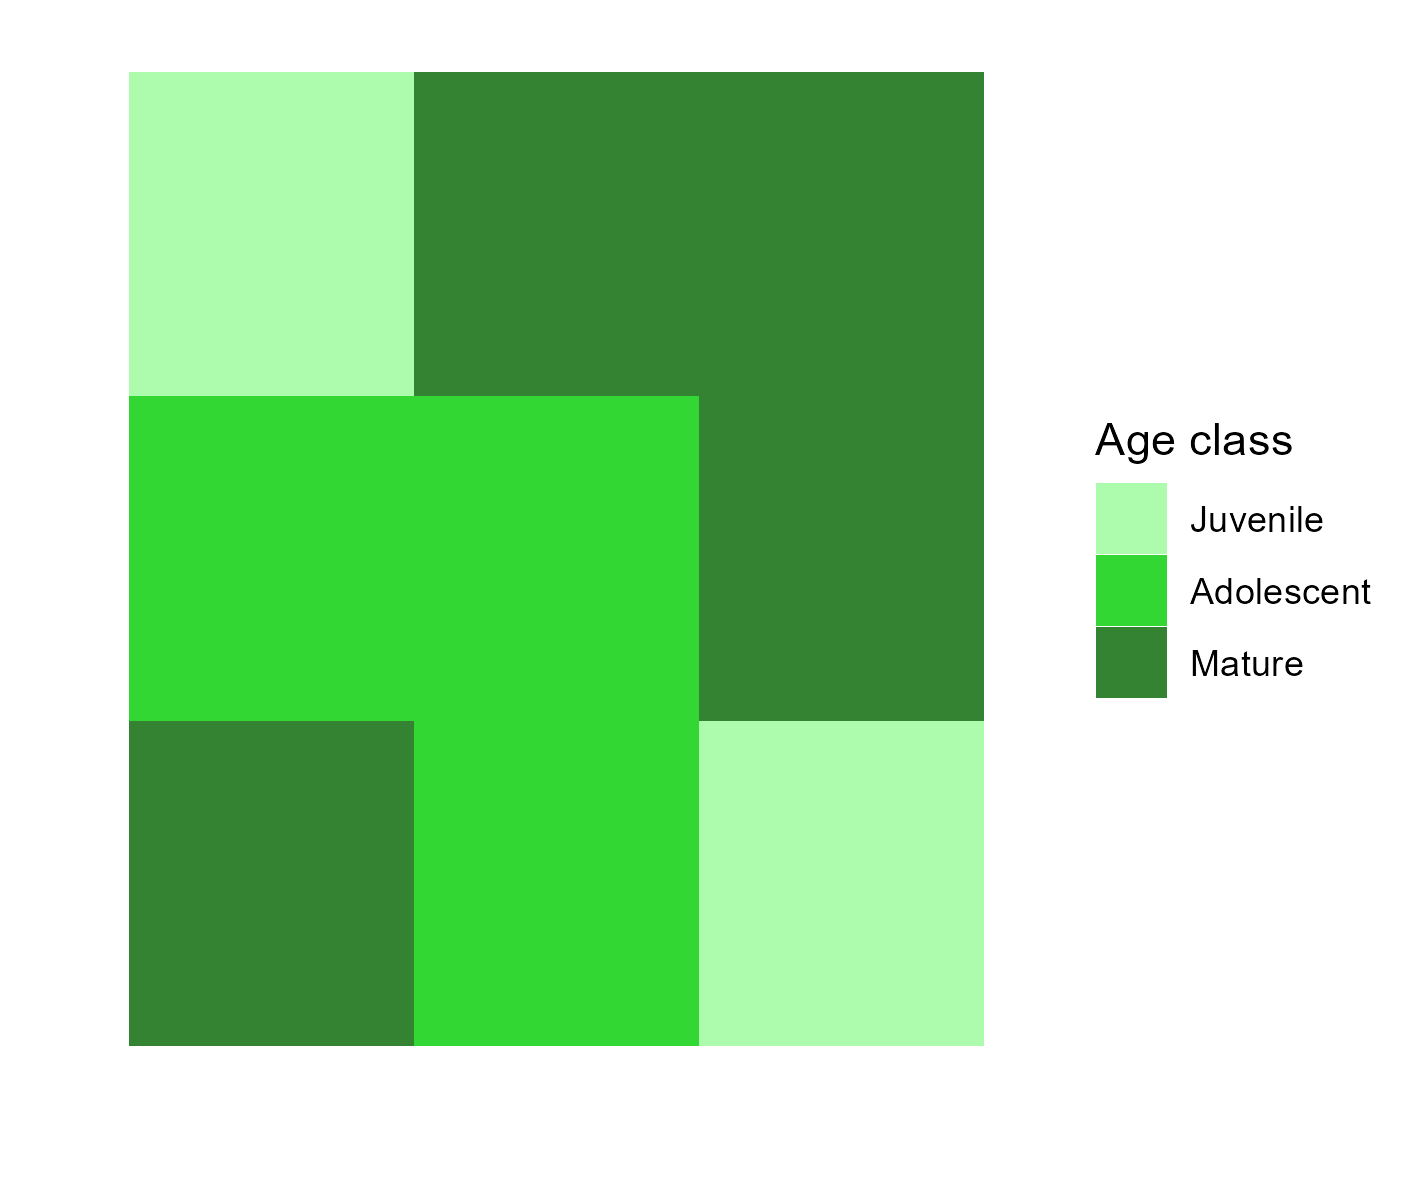
\includegraphics[width = .28\textwidth]{figures/wildland/illustration_from_raster.png}\\
    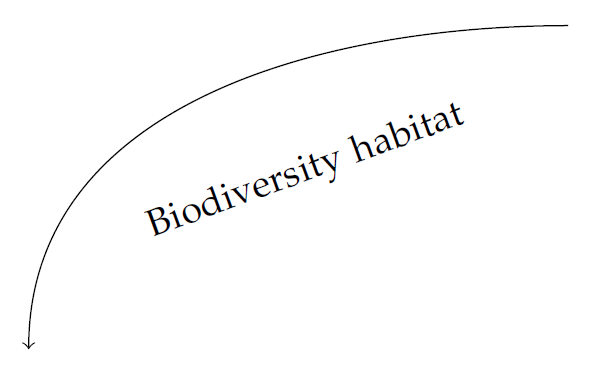
\includegraphics[width = 0.2\textwidth]{figures/wildland/arrow_biod2.PNG}
    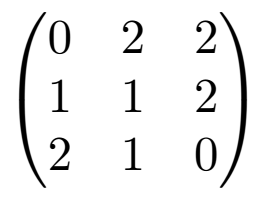
\includegraphics[width = 0.18\textwidth]{figures/wildland/land3.PNG}
    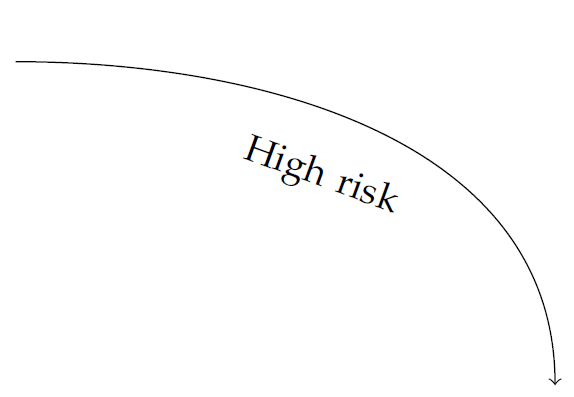
\includegraphics[width = 0.2\textwidth]{figures/wildland/arrow_fuel2.PNG}
    \\
    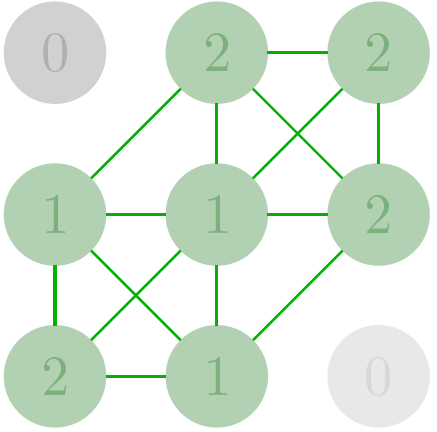
\includegraphics[width=0.2\textwidth]{figures/wildland/biodiv_3.PNG} \hspace*{4cm}
    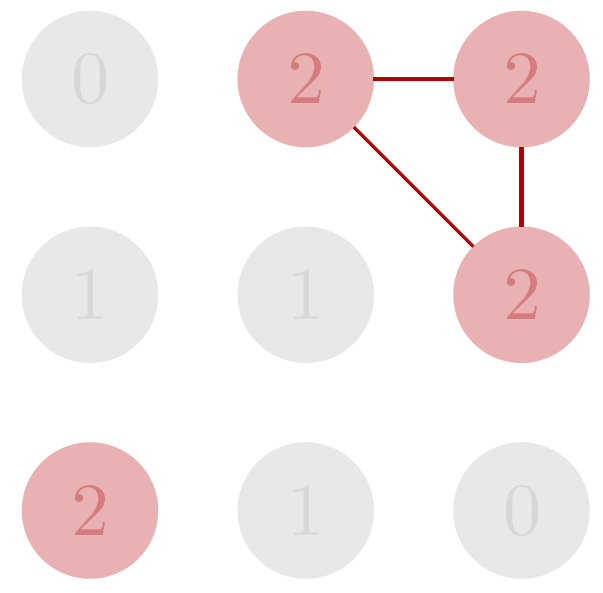
\includegraphics[width=0.2\textwidth]{figures/wildland/fire_3.PNG}\\
    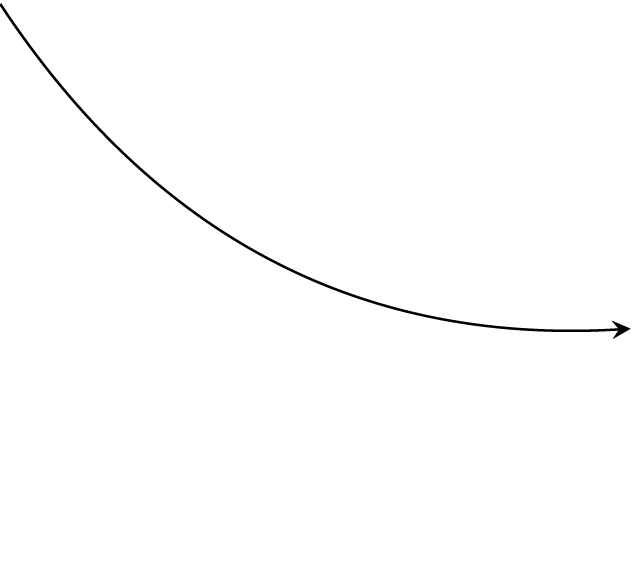
\includegraphics[width=0.18\textwidth]{figures/wildland/arrow_right.PNG}
    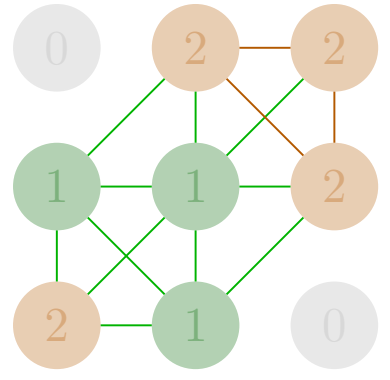
\includegraphics[width = 0.2\textwidth]{figures/wildland/graphe_feu_biod_33.PNG}
 	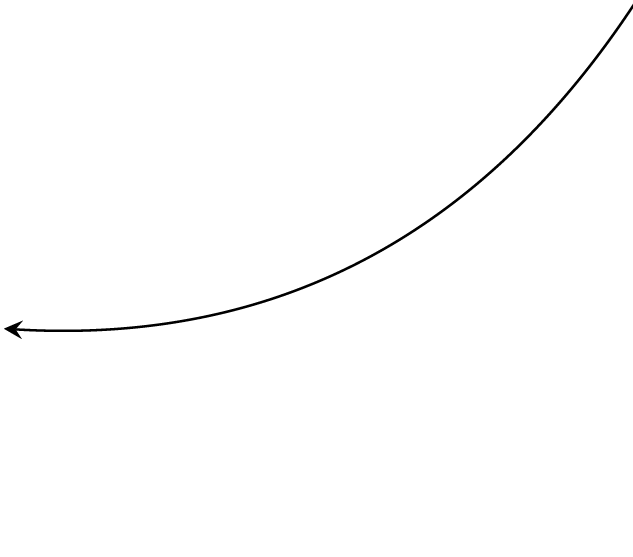
\includegraphics[width=0.18\textwidth]{figures/wildland/back_left.PNG}
    \caption{Illustration of the suitable habitat and high risk graphs for $n=3$}
    \subcaption*{The first layer is the values from a raster $\mathbf{A}_t$ of age classes in a forest landscape. It is turned into two different graphs. \\
In the left graph, the green vertices are $V_{\mathcal{B}_t}$ and support biodiversity habitat, while on the right graph, red vertices are $V_{\mathcal{F}_t}$ display high risk. Green and red links are respectively $E_{\mathcal{B}_t}$ and $E_{\mathcal{F}_t}$ \\
The high risk graph has two components (top right corner with 3 nodes, and bottom left corner with 1 node), while the biodiversity habitat graph only has one. \\
Cells for which the value is 0 are not considered as nodes for both graphs, and are thus not connected to the rest of the graphs. 
\\
In the final lansdcape, because $\mathcal{F}_t\subset \mathcal{B}_t$, the landscape  where orange cells are high fuel load and also support biodiversity habitat (e.g. $a_{ijt} \in V_{\mathcal{B}_t} \cap V_{\mathcal{F}_t}$)}
    \label{fig:graph_overlap}
\end{figure}

To assess the connectivity of $\mathcal{F}_t$ and $\mathcal{B}_t$, we use a global connectivity indicator. As connectivity can be measured in numerous ways in graph theory, we use this metric as is satisfies criteria pertaining to its evolution when vertices and edges are removed \citep{pascual-hortal_comparison_2006} when using graph theory applied to landscape ecology. Additionally, it offers a reformulation of the metric used in previous work closedly related to ours \citep{minas_spatial_2014, rachmawati_optimisation_2016} (see appendix \ref{sec:connectivity} for a demonstration). We define the global connectivity index of a given graph $\mathcal{G} = (\mathcal{V}, \mathcal{E})$ as\footnote{With $card$ being the cardinal operator in set theory and denotes the number of elements in a set}:
\begin{equation}
H(\mathcal{G}) = card(V) + 2card(E)
\label{eq:high_connectivity}
\end{equation} 
Let a \textit{patch} be a collection of connected cells of suitable wildlife habitat.
This indicator considers that a habitat cell is connected to itself (i.e, within a habitat patch, there is no barrier) and whether it is connected to other cells.  
It implies lower connectivity when the distance between habitat cells increases, attains its maximum value when a single habitat patch covers the whole landscape, indicates lower connectivity as the habitat is progressively more fragmented, considers negative the loss of a connected or isolated cell, and detects as more important the loss of bigger patch, and less important steppingstone cells or patches. 
\\
Our global connectivity indicator is similar to the notion of \textit{energy of a graph} \citep{gutman_energy_2001}, which can be understood as a measure of connectedness (highly connected graphs tend to have high energy) for graphs. However, we differ from \cite{gutman_energy_2001} by including self-loops as habitat cells and patches are connected to themselves. Our formulation of $H$ reframes a quadratic form from the adjacency matrix of a graph grid structure (appendix \ref{sec:connectivity}). The adjacency matrix displays interaction among nodes that are neither purely constructive or destructive, as some combinations of active neighboring nodes will add to global connectivity, while other combinations may substract global connectivity. In all the landscape sizes we used, eigenvalues of the adjacency matrix were both positive and negative, leading to indefiniteness (see figure \ref{fig:eigenvalues}). Therefore, $H$ is not globally convex nor concave. 
\\
%and The vertices of $\mathcal{B}_t$ are cells that are at suitable habitat status (e.g. $Habitat(a_{it})=1$ and high risk status (e.g. $Risk(a_{it})=1$) and suitable habitat status
%
%We transform $A_t$ the set of cells constituting the landscape into graphs $G_t$ whose vertices $V_t$ (or nodes) are the cells in the landscape, and edges $E_t$ represent the connections between cells. We partition the landscape in two graphs, $G_{B_t}$ and $G_{F_t}$, each describing the network of mature habitat and risky patches (see fig. 1 for a representation). Landscape ecology has long used numerous, theoretically grounded indicators to analyze landscapes 
%
%\citep{urban_landscape_2001,minor_graph-theory_2008}. We use a global connectivity indicator that satisfies \cite{pascual-hortal_comparison_2006} criteria, grounded in graph theory, that offer a reformulation of \cite{rachmawati_optimisation_2016} (see Appendix \ref{sec:connectivity}). 
%Figure reference : \ref{fig:graph_overlap}
%
%We define cells to be connected if (i) they are within an 8-cell neighborhood and (ii) share the same status e.g. for a cell $i$, if cell $j$ is an 8-cell neighborhood (should we define it?)
%
%We define the global connectivity index of habitat and risky patches in landscape $A(t)$ as:
%
%This indicator considers that a habitat patch is connected to itself (i.e, within a habitat patch, there is no barrier) and whether it is connected to other patches.  
%It implies lower connectivity when the distance between patches increases, attains its maximum value when a single habitat patch covers the whole landscape, indicates lower connectivity as the habitat is progressively more fragmented, considers negative the loss of a connected or isolated patch, and detects as more important the loss of bigger patches, of key and less important steppingstone patches.
%
%We use a connectivity matrix to evaluate the ladnscape such that ...
%\textit{note that the framework is robust to changing the dispersal abilities. For example, one could think of (i) changing the dispersal abilities and (2) increase the size of the landscape to run applied stuff and (3) finding metrics to prioritize over species with different dispersal abilities. \textbf{This is a good discussion point : next work should include a variety of dispersal abilities and contributions to functional diversity to really dig deeper in this issue. }}
%\\\\

\subsection{Social planner decision : the high-risk /connectivity dilemma}
\subsubsection{Dynamic decision problem}
A social planner tries to minimize the global connectivity index of the high risk graph, using fuel treatments (eq. \ref{eq:objective}). However, when implementing treatment, a cell's successional stage is reset to \textit{juvenile}, thus destroying biodiversity habitat. In coherence with real world applications, the social planner is faced with a temporal budget constraint (e.g. the sum of treatments $\sum_{ij}x_{ijt}$ must be lower or equal to the $Budget$ - eq. \ref{const:budget}) as well as an ecological constraint, in terms of biodiversity habitat connectivity (e.g. the global connectivity of biodiversity habitat $H(\mathcal{B}_t)$ must be larger than constraint $Biod$ - eq. \ref{constr:biod}). Both the ecological and budget constraint need to be satisfied in each period.
\\
For the sake of the analysis, we focus on two layers of complexity : time and space. We do not include a stochastic component related to wildfire risk e.g. we adopt a deterministic framework where the value at risk (global connectivity of risky cells) is weighed against the loss in biodiversity habitat connectivity. Additionally, we consider a homogeneous distribution of treatment costs across the landscape e.g. cost of treatment in each cell through time is $1$. We come back to this assumption in the discussion. Monetary benefits are also homogenously distributed across the landscape, and normalized to 1. Note that there is, however, heterogeneous returns to treating across the landscape : some cells will contribute more than other to global connectivity. Finally, given that the planning horizon is finite, we do not discount future high risk connectivity scores and assume each period is equally important in decision making.

The optimization problem is : 

\begin{align}
    \min_{ \{\{x_{ijt}\}_{(i,j)}\}_{t=1}^T} & \left[ \sum_{t=1}^T H(\mathcal{F}_t)\right] \label{eq:objective}\\
\text{Such that: } & \notag \\
\mathbf{A}_0 &\text{ given} \label{eq:init_cond}\\
\forall t \in \{1, ..., T\} : & \notag \\
H(\mathcal{B}_t)&\geq Biod,\text{  }\label{constr:biod}\\
\text{ and }\forall (i,j) \in \{1,...,n\}   :& \notag \\
a_{ijt+1}& = \min((a_{ijt+1}(1-x_{ijt});2), \label{const:dyn}\\
 \sum_{i,j} x_{ijt} & \leq Budget,\text{  } \label{const:budget}\\
x_{ijt}&\in \{0,1\}\label{const:control}
\end{align}

\begin{table}[h]
\centering
\onehalfspacing
\begin{tabular}{|c|c|}
\hline
Notation & Concept \\
\hline \hline
$\mathbf{A}_t$ & Landscape matrix representing successional stage at time $t$ \\
$a_{ijt}$ & Cell $(i,j)$ of landscape with value $\in \{0,1,2\}$\\ 
$x_{ijt}$ & Treatment status $\in\{0,1\}$ of cell $(i,j)$ at time $t$ \\
$H$ & Global connectivity measure\\
$\mathcal{F}_t = (V_{\mathcal{F}_t}, E_{\mathcal{F}_t})$ & Graph of high risk cells\\
$\mathcal{B}_t = (V_{\mathcal{B}_t}, E_{\mathcal{B}_t})$ & Graph of suitable habit cells\\
\hline \hline
$Biod \in \{0,...,\max H(\mathcal{B})\}$ & Level of habitat global connectivity constraint\\
$Budget \in \{1,2,3,4\}$ & Level of the budget constraint\\
$n \in \{3,4,100\}$ & Size of the lansdcape\\
$c = 3$ & Number of age classes \\
$T \in \{5,10\} $ & Planning horizon\\
\hline 
\end{tabular}
\caption{Summary of model variables and functions}
\end{table}
%There are several reasons for this choice. First, the complexity of our problem is increasing in space and time, and in the number of initial conditions, as interpolation in a spatial setting is difficult given the behavior of our objective function. 
As common in the literature, we can express the budget as a share of land being treated ranging from 10\% to 33\% of the surface area (when $n=3$) and 5 to 25\% of the surface area (when $n=4$). These values encompass historical and projected policies in Australia \citep{burrows2013}, the United States \citep{GAO2019} and Southern Europe \citep{Fernandes2013}.
\\
Additionally, we solve the problem for a range of possible habitat connectivity values, ranging from $0$ to the maximum possible habitat connectivity for each landscape size $n$.

\subsubsection{Non-convexity and dimensionality curse}
Our problem can be classified as a \textit{critical node detection problem}, i.e, a problem of locating the vertices that best degrade our global connectivity metric $H(\mathcal{F}_t)$ \citep{ARULSELVAN20092193}. Problems of the critical node class are computationally difficult (e.g. NP - Hard) in a single graph \citep{ARULSELVAN20092193, matsypura_wildfire_2018}. Efficient heuristics to find near-optimal solutions exist and leverage perturbations around local solutions \citep{ARULSELVAN20092193, Zhou2017}. Compared to the canonical \textit{critical node detection} problem, our problem features a non-convex objective function, a budget constraint, and a constraint on habitat connectivity, which imposes a constraint on the supergraph of high risk cells. Given our constraints, the behavior of the global connectivity measure $H$, standard optimization techniques cannot be applied, and heuristics are required. \\
%We solve the dynamic, integer program of the landscape manager
In dynamic problems, a standard technique is dynamic programming \citep{Bellman}. Dynamic programming provides a temporal decomposition of the initial problem defined over $T$ periods, into $T$ recursive problems, as it relies on the 'optimality principle'\footnote{"An optimal policy has the property that whatever the initial state and initial decision are, the remaining decisions must constitute an optimal policy with regard to the state resulting from the first decision". (See \cite{Bellman}, Chap. III.3., p.83)"}. A value function $V$, mapping each possible state of the world e.g. $\mathbf{A}_t$ to the optimal value of the objective function along the planning horizon, is iterated upon to find the optimal policies $x_{ijt}^*(\mathbf{A}_t)$, i.e, the sequence of optimal treatments, and the optimal states $\mathbf{A}_t^*(\mathbf{A}_0)$ resulting from the optimal policies and the initial conditions.
However, it is impractical in our case. Our problem suffers a \textit{dimensionality curse} \citep{Bellman}. There are $3^{n^2}$ values for the state variables \footnote{Given that the landscape $\mathbf{A}$ is of size $n\times n$, and that each element of $a_{ij}$ can take $c=3$ values, there are $3^{n^2}$ landcape configurations possible} in each period and the specific nature of our objective function $H$, the habitat connectivity and budget constraints make interpolation of a value function impossible \footnote{As a matter of fact, with a large number of state variables e.g. a high-dimensional state space, methods such as adaptive sparse grids can be used towith smooth, continuous objective functions \citep{brumm_adaptive_2017} to circumvent the dimensionality curse. The fact that the input space is an $n^2$-dimensional binary Cartesian product and that $H$ is not globally convex hinder the use of such tools.}.
%To manage the expected damages resulting from wildfires, the land planner can decide to undertake specific treatments, in the form of a combination of controlled burns and/or mechanical thinnings. Upon treatment, we assume that vegetation age in the cell is reset to 'absent': the wildfire risk vanishes, but so does the habitat and its connection to surrounding cells. Given the tension between maintaining habitat and reducing wildfire risk, the land planner aims to minimize a deterministic measure of connectivity of the high fuel loads in the landscape while maintaining a given level of biodiversity habitat connectivity under a budget constraint, over a planning horizon of length $T$. 
%For the sake of the analysis, we focus on two layers of complexity over time and space: global connectivity of high risk and biodiversity habitat. We do not consider stochastic wildfire behavior\textbf{point on risk and expected utility? } , heterogeneity in the economic costs or benefits (i.e, homogeneous treatment costs and no patch-specific asset to protect). The framework is however amenable to such a prioritization. We also assume that the budget cannot be banked, and has to be utilized in each period, consistent with operational rules. Moreover, as the budget is constrained in each period, the measure of risk is bounded and the planning horizon is finite, we rule out discounting and assume each generation matters as much to the social planner. 
%We abstract from decision-making in a risky environment, as it has been extensively described in economics and decision theory \citep{Mouysset2013}. Moreover, we mimic the role of risk aversion by varying the level of habitat connectivity constraint the decision maker chooses. 
%If ignition is a binary process in each period, the probability of which is independent of the high-risk graph properties, our model can be viewed as minimizing an upper bound of the expected losses from wildfires (see appendix).


\subsection{Solution method and computational experiments}

Three key features of our problem hint that a dynamic (e.g. that optimizes the objective function over the whole planning horizon) and a repeated myopic solution (e.g. which optimizes the objective function in each period)  should be similar. The dynamics occur before the decision is made, therefore the decision maker has full knowledge about the state of the system. The dynamics are simplified and have relatively little depth, as we limit ourselves to 3 age classes. Finally, our intertemporal objective function is additively separable.

Our solution methods resorts to two key ingredients : optimization heuristics, and comparison between the dynamic and repeated myopic problem. \\
First, we circumvent the non-convexity of the global connectivity metric and the high dimension of the state space by using a genetic algorithm \citep{holland_adaptation_1975} (implemented in \textsf{R} with package \textit{GA} \citep{GA_2017}) for 300 randomly generated landscapes, with population size of $200$ and $250$ iterations. Genetic algorithms are especially suited for high dimensional, combinatorial search spaces\footnote{Here, the control variable is a $Tn^2 = 5n^2$ binary variable} and fare better than a brute force approach, or other heuristics (Particle Swarm Optimization or Simulated Annealing). 
\\
Then, we compare the performance of a 5-period objective function to a 5 period repetition of a static objective function. We trade the completeness of dynamic programming for a more manageable approach, where we compare these approaches for $696$ and $884$ randomly drawn landscapes of size $n \in \{3,4\}$. We sample the landscapes according to the distribution of possible landscapes (see figure \ref{fig:appendix_distribution}). As landscapes with large numbers of \textit{juvenile} and \textit{adolescent} cells are overrepresented, we impose that underrepresented possible landscapes are included at least 2 times in our sample, to disentangle composition (e.g. number of cells of each successional stage) from configuration (location of cells) effects.

 We focus $T=5$ planning horizon for several reasons. First, as the dynamic of our ecological processes comprises 3 stages, using a 5-period horizon allows for each cell to grow from its original stage to \textit{mature}, be treated, and revert to its original stage, e.g. allows for a full successional cycle to be performed. Second, a 5-period horizon corresponds to a long policy horizon, ranging from 25 years to 200 years \citep{mccoll_gausden_pathways_2019, thomas_wildlife_1979}.
Third, for our approach to be useful for policy making given that we abstract from stochastic modifications to the environment (e.g. occurence of wildfire, spread of invasive species increasing flamability at a given age etc), policies need to be forward looking with enough temporal depth to be relevant and be reevaluated with potentially new initial conditions resulting from environmental perturbations.\\
Next, we increase the size of our sample with repeated static optimization and temporal depth, to encompass all the possible landscape configurations for landscape size $n \in \{3, 4\}$, over the whole range of possible values for the biodiversity habitat constraint, over $T=10$ years. 
Of all the $3^{n^2}$ initial landscapes combinations possible, we only keep landscapes that are unique up to a permutation\footnote{That is to say, landscape $\mathbf{A}_0$ is included in the set of initial conditions $\mathcal{I}$ if and only if for any element $\mathbf{A'}_0$ in $\mathcal{I}$, $\mathbf{A}_0$ is not a permutation (eg can be obtained through rotations or symmetries) of $\mathbf{A'}_0$}. This results in a sharp reduction of landscapes to consider, from $19,683$ initial conditions to $2861$ unique initial landscapes for $n=3$, and from $43,046,721$ initial to $5,398,082$ unique initial landscapes for $n=4$. We focus on exact optimal solutions for all the initial conditions of these small-scale landscapes and implement our own solution algorithm in Python 3.9.13 and R 4.3.3\footnote{Data and code are \href{https://github.com/sim-jean/Landscape_connectivity_dilemma}{publicly available}}.
\\
Third, we increase the landscape size to $n=100$, for a sample of 20 large scale (10,000 cells) landscapes with varying compositions and autocorrelation using two-dimensional fractional Brownian motions  (table \ref{tab:composition_nlm} summarizes their characteristics and figure \ref{fig:ex_nlm} illustrates 6 of them). We use neutral landscape models \citep{caswell_community_1976, gardner_neutral_2007} and implement them in \textsf{R} \citep{sciaini_nlmr_2018}. Neutral landscape models were designed in theoretical landscape ecology to develop spatial ecology indicators and ``evaluate the effects of landscape structure on ecological processes'' \citep{with_neutral_1997}. Even though they are designed as null models to compare with real landscapes, after ecological processes have shaped them, they provide a useful basis for scaling our analysis. We solve the repeated myopic optimization problem on these 20 landscapes over $T=10$ periods.\\
%
%
%\subsubsection{Non-convexity and dimensionality curse}
%Our problem can be classified as a \textit{critical node detection problem}, i.e, a problem of locating the vertices that best degrade our global connectivity metric $H(\mathcal{F}_t)$ \citep{ARULSELVAN20092193}. Problems of the critical node class are computationally difficult (e.g. NP - Hard) in a single graph \citep{ARULSELVAN20092193, matsypura_wildfire_2018}. Efficient heuristics to find near-optimal solutions exist and leverage perturbations around local solutions \citep{ARULSELVAN20092193, Zhou2017}. Compared to the canonical \textit{critical node detection} problem, our problem features non-convex objective function, a budget constraint, and a constraint on habitat connectivity, which imposes a constraint on the supergraph of high risk cells. Given our constraints, the behavior of the global connectivity measure $H$, standard optimization techniques cannot be applied. \\
%We solve the dynamic, integer program of the landscape manager
%In dynamic problems, a standard technique is dynamic programming. Dynamic programming provides a temporal decomposition of the initial problem defined over $T$ periods, into $T$ recursive problems, as it relies on the 'optimality principle'\footnote{"An optimal policy has the property that whatever the initial state and initial decision are, the remaining decisions must constitute an optimal policy with regard to the state resulting from the first decision". (See \cite{Bellman}, Chap. III.3., p.83)"}. A value function $V$, mapping each possible state of the world e.g. $\mathbf{A}_t$ to its objective function value, is iterated upon to find the optimal policies $x_{ijt}^*(\mathbf{A}_t)$, i.e, the sequence of optimal controlled burns, and the optimal states $\mathbf{A}_t^*(\mathbf{A}_0)$ resulting from the optimal policies and the initial conditions.
%However, it is impractical in our case. As a matter of fact, our problem suffers a \textit{dimensionality curse} \citep{Bellman}. There are $3^{n^2}$ possible combinations\footnote{Given that the landscape $\mathbf{A}$ is of size $n\times n$, and that each element of $a_{ij}$ can take $c=3$ values, there are $3^{n^2}$ landcape configurations possible} in each period and the specific nature of our objective function $H$, the habitat connectivity and budget constraints make interpolation of a value function impossible \footnote{As a matter of fact, even with a large number of state variables e.g. a high-dimensional state space, adaptive sparse grids can be used with smooth, continuous objective functions \citep{brumm_adaptive_2017}. The fact that the input space is an $n^2$-dimensional binary Cartesian product and that $H$ is not globally convex hinder the use of such tools.}. 
%
%Nonetheless, three key features of our problem hint that dynamic and repeated myopic solutions should be similar. The dynamics occur before the decision is made, therefore the decision maker has full knowledge about the state of the system. The dynamics are simplified and have relatively little depth, as we limit ourselves to 3 age classes. Finally, our intertemporal objective function is additively separable.
%
%
%
%\subsubsection{Dynamic v. repeated myopic solutions}
% 
%To circumvent this issue, we adopt a three-fold approach. \\
%First, we trade the completeness of dynamic programming (e.g. solution of the problem for the entire domain of the state variable $\mathbf{A}$) for a manageable piecemeal approach, where we solve the complex 5-period combinatorial problem with a genetic algorithm \citep{holland_adaptation_1975} (implemented in \textsf{R} with package \textit{GA} \citep{GA_2017}) for 300 randomly generated landscapes, with population size of $200$ and $250$ iterations. Genetic algorithms are especially suited for high dimensional, combinatorial search spaces\footnote{Here, the control variable is a $Tn^2 = 5n^2$ binary variable} and fare better than a brute force approach, or other heuristics (Particle Swarm Optimization or Simulated Annealing). 
%
%Three key features of our problem hint that dynamic and repeated myopic solutions should be similar. The dynamics occur before the decision is made, therefore the decision maker has full knowledge about the state of the system. The dynamics are simplified and have relatively little depth, as we limit ourselves to 3 age classes. Finally, our intertemporal objective function is additively separable.
%Hence, we compare the performance of the 5 period, genetic algorithm approach to a repeated static optimization procedure, for landscapes of size $n\in\{3,4\}$. While this size appears simplifying, it encapsulates the main mechanisms displayed in similar models \citep{rachmawati_optimisation_2016, rachmawati_fuel_2018}. Based on these results, we increase the planning horizon to
%\\
%\textbf{Comment est ce qu'on dit ici qu'on accroit peut être l'horizon?}
%Second, we perform a repeated static optimization on all the possible landscape configurations for landscape size $n \in \{3, 4\}$, over all the whole range of possible values for the biodiversity habitat constraint, over 5 years. This approach sacrifices the dynamics of our problem but allows us to scan the entire state space to gain insights.
%Of all the $3^{n^2}$ initial landscapes combinations possible, we only keep landscapes that are unique up to a permutation\footnote{That is to say, landscape $\mathbf{A}_0$ is included in the set of initial conditions $\mathcal{I}$ if and only if for any element $\mathbf{A'}_0$ in $\mathcal{I}$, $\mathbf{A}_0$ is not a permutation (eg can be obtained through rotations or symmetries) of $\mathbf{A'}_0$}. This results in a sharp reduction of landscapes to consider, from $19,683$ initial conditions to $2861$ unique initial landscapes for $n=3$, and from $43,046,721$ initial to $5,398,082$ unique initial landscapes for $n=4$. We focus on exact optimal solutions for all the initial conditions of these small-scale landscapes and implement our own solution algorithm in Python 3.9.13 and R 4.3.3\footnote{Data and code are \href{https://github.com/sim-jean/Landscape_connectivity_dilemma}{publicly available}}.
%\\
%Third, we simulate 20 large scale (10,000 cells) landscapes with varying compositions and autocorrelation using two-dimensional fractional Brownian motions  (table \ref{tab:composition_nlm} summarizes their characteristics and figure \ref{fig:ex_nlm} illustrates 6 of them). We use neutral landscape models \citep{caswell_community_1976, gardner_neutral_2007} and implement them in \textsf{R} \citep{sciaini_nlmr_2018}. Neutral landscape models were designed in theoretical landscape ecology to develop spatial ecology indicators and ``evaluate the effects of landscape structure on ecological processes'' \citep{with_neutral_1997}. Even though they are designed as null models to compare with real landscapes, after ecological processes have shaped them, they provide a useful basis for scaling our analysis. We solve the repeated myopic optimization problem on these 20 landscapes.
%
%using dynamic programming. Dynamic programming provides a temporal decomposition of the initial problem defined over $T$ periods, into $T$ recursive problems, as it relies on the 'optimality principle'\footnote{"An optimal policy has the property that whatever the initial state and initial decision are, the remaining decisions must constitute an optimal policy with regard to the state resulting from the first decision". (See \cite{Bellman}, Chap. III.3., p.83)"}.  The outputs of the method are both the optimal policies $x_j^*(t,A)$, i.e, the sequence of optimal controlled burns, and the optimal states $A_j^*(t,A_0)$ resulting from the optimal policies and the initial conditions. Moreover, we solve a repeated myopic optimization procedure, where in each time step, the decision maker minimizes the current global connectivity measure of high risk cells, under constraints \ref{eq:init_cond}-\ref{const:control}. In the dynamic problem, the biodiversity habitat and budget constraints gradually restrict the solution space, and limit the extent to which system dynamics (e.g the appraisal of long terms successional stages across the landscape) may impact optimal solutions. We compare the repeated myopic solution to the dynamic solution.
%
%\subsubsection{Circumventing non-convexity and dimensionality curse}
%
%Our problem can be classified as a \textit{critical node detection problem}, i.e, a problem of locating the vertices that best degrade our global connectivity metric $H(\mathcal{F}_t)$ \citep{ARULSELVAN20092193}. Problems of the critical node class are computationally difficult (e.g. NP - Hard) in a single graph \citep{ARULSELVAN20092193, matsypura_wildfire_2018}. Efficient heuristics to find near-optimal solutions exist and leverage perturbations around local solutions \citep{ARULSELVAN20092193, Zhou2017}. Our problem is a constrained, integer optimization problem with a non-convex objective function,
%that constrains not only the set of nodes to be removed but also metrics relative to a larger graph structure e.g. the supergraph of high risk cells, biodiversity habitat. Given the behavior of the global connectivity measure $H$, standard optimization techniques cannot be applied. \\
%Additionally, the complexity of our combinatorial problem increases with landscape size $n$, the number of vegetation age classes $c$, and time $T$ i.e. features a \textit{dimensionality curse} \citep{Bellman}: there are $c^{n^2}$ eg. $3^{n^2}$ initial landscape configurations possible, and given an initial landscape, there are $n^2 \times T$ possible treatment allocations to be considered. 
%To circumvent these issues, we use a genetic algorithm \citep{holland_adaptation_1975} (implemented in \textsf{R} with package \textit{GA} \citep{GA_2017}). Compared to other heuristics, such as Particle Swarm Optimization or Simulated Annealing, genetic algorithms fare better on high dimension, combinatorial search spaces. With small scale landscapes (e.g. $n\in \{3,4\}$), we use a population size of $100$ individuals with $250$ iterations which guarantees that the heuristic converges to a near optimal solution.
%
%Moreover, as the objective function is neither globally convex nor concave, and the structure of the optimization problem is constrained, we required large test populations for our genetic algorithm to avoid getting stuck in local minima.  es.
%
%\subsubsection{Small and large scale repeated myopic optimization}
%
%We limit ourselves to studying the initial conditions in landscapes of size $n=3$ and $4$. While this formulation appears simplifying, it encapsulates the main mechanisms displayed in similar models \citep{rachmawati_optimisation_2016, rachmawati_fuel_2018}.\\
%First, we solve the dynamic problem and repeated static problem for 300 randomly selected initial landscapes.
%Then, we focus on all the possible landscape combinations of size $n \in \{3,4\}$ using repeated myopic optimization, over all the whole range of possible values for the biodiversity habitat constraint, over 5 years. \\
%Of all the $3^{n^2}$ initial landscapes combinations possible, we only keep landscapes that are unique up to a permutation\footnote{That is to say, landscape $\mathbf{A}_0$ is included in the set of initial conditions $\mathcal{I}$ if and only if for any element $\mathbf{A'}_0$ in $\mathcal{I}$, $\mathbf{A}_0$ is not a permutation (eg can be obtained through rotations or symmetries) of $\mathbf{A'}_0$}. This results in a sharp reduction of landscapes to consider, from $19,683$ initial conditions to $2861$ unique initial landscapes for $n=3$, and from $43,046,721$ initial to $5,398,082$ unique initial landscapes for $n=4$. We focus on exact optimal solutions for all the initial conditions of these small-scale landscapes and implement our own solution algorithm in Python 3.9.13 and R 4.3.3\footnote{Data and code are \href{https://github.com/sim-jean/Landscape_connectivity_dilemma}{publicly available}}.
%
%
%
%Finally, we simulate 20 large scale (10,000 cells) landscapes with varying compositions and autocorrelation using two-dimensional fractional Brownian motions  (table \ref{tab:composition_nlm} summarizes their characteristics and figure \ref{fig:ex_nlm} illustrates 6 of them). We use neutral landscape models \citep{caswell_community_1976, gardner_neutral_2007} and implement them in \textsf{R} \citep{sciaini_nlmr_2018}. Neutral landscape models were designed in theoretical landscape ecology to develop spatial ecology indicators and ``evaluate the effects of landscape structure on ecological processes'' \citep{with_neutral_1997}. Even though they are designed as null models to compare with real landscapes, after ecological processes have shaped them, they provide a useful basis for scaling our analysis. We solve the repeated myopic optimization problem on these 20 landscapes.
%
%
\subsection{Lanscape indicators}
\label{section:indicators}
To characterize the managed landscapes, we mobilize several indicators from landscape ecology and graph theory (see appendix \ref{sec:appendix_wildland__indicators}).

First, we account for the high risk and habitat surfaces in the landscape by measuring the number of vertices in each graph.
Second, to assess landscape connectivity and fragmentation as well as landscape diversity\footnote{In the context of fire prone ecosystems, the notion of ``fire mosaics'' \citep{bradstock_which_2005} conveys the idea that fire causes variations in successional stages through space thus providing different types of habitat for biodiversity and improving biodiversity}, we use our global connectivity metric $H$ (eq. \ref{eq:high_connectivity}), as well as the \textit{number of components}\footnote{A \textit{component $\mathcal{C}_t$} of graph $\mathcal{G}_t$ is a maximally connected subgraph of $\mathcal{G}_t$ that is not part of any larger connected subgraph. A component is \textit{connected} (for all two vertices $(u,v) \in V_{\mathcal{C}}$, there exists a path in $\mathcal{C}_t$ that connects them) and $\mathcal{C}_t$ being a subgraph of $\mathcal{G}_t$, it is \textit{maximal} if there is no other connected subgraph $\mathcal{C'}$ of $\mathcal{G}_t$ such that $\mathcal{C}_t$ is a proper subgraph of $\mathcal{C'}_t$. Figure \ref{fig:graph_overlap} illustrates this concepts in both the habitat and high risk graphs resp. $\mathcal{B}_t$ and $\mathcal{F}_t$}.
To specifically assess landscape diversity, we use the Simpson index \citep{simpson_measurement_1949} on successional stages stages (eq. \ref{eq:simpson})\footnote{Similar results can be found with the Shannon index \citep{Shannon1949}. To avoid issues related to degenerate values and logarithms, we focus on the Simpson index.}. 
However, the Simpson index does not account for the diversity of spatial patterns: a checkered landscape with two seral stages would be as diverse as a landscape with two large patches for each seral stage, according to the Simpson index. Therefore, we use the landscape shape index (eq. \ref{eq:LSI}), a normalized ratio between the perimeter of biodiversity habitat and its area \citep{patton_diversity_1975, McGarigal_1995}.
%\begin{equation}
%LSI = \frac{perimeter(\mathcal{G}_t)}{4n} \text{ such that }\mathcal{G}_t \in \{\mathcal{B}_t,\mathcal{F}_t\}
%\end{equation}
To disentangle the correlated effects of perimeter and area that affect the landscape shape index, we use a successional stage heterogeneity index, that averages the probability that, for each cell, neighbors in the 4 cardinal directions share the same successional stage (eq. \ref{eq:lth_index}). The index ranges between 0, when the successional stage is the same across the whole landscape, to 1, in a checkered landscape. The index assesses whether the landscape is a mosaic \citep{bradstock_which_2005}, and if it displays structural diversity, conducive to diverse communities and functional diversity. 

\section{Results}
\label{section:results}
\begin{itemize}
\item Need to rethink the argument in terms of steady states
\\
$\Rightarrow$ We no longer can use this argument because we sacrificed the duration
\item We want to characterize the long term trajectories with $T=5$?
\item What can we do?
\end{itemize}
\subsection{Steady states}
Our simulations show that 100\% of the initial landscapes converge in finite time towards a steady state solution, that minimizes wildfire risk while satisfying budgetary and habitat connectivity requirements. Steady states are landscape cycles with finite periods. Analyzing the steady-state cycles (and the unique landscapes that form them) drastically reduces the set of landscapes to analyze: they represent 2\% (resp. $0.001\%$) of the initial landscapes of size $n=3$ (resp. $n=4$). Our model highlights the convergence of landscapes towards types that can be managed to deliver several objectives. As landscape size increases, the number of steady state landscape cycles increases, but the power of convergence increases as well (e.g. ratio between initial configurations and effective steady state landscapes): from 19 683 initial landscapes when $n=3$, 51 steady states emerge and from 43 046 721 initial landscapes when $n=4$, at most 95 diverse steady-state landscapes emerge. Focusing on steady states makes all the more sense as landscape size increases. 

Eventually, figure \ref{fig:distrib_cycles} shows that conditional on data availability on every patch, the more the decision maker wants to conserve biodiversity, the fewer steady-state landscapes she has to consider. An increase in the habitat requirement reduces the room for maneuver. Indeed, budget acts as a complexifying factor: the larger the budget (relative to costs), the larger the set of steady-states to consider. 
%Our results show that habitat connectivity can be an objective and serve as an information cost-saving strategy. Data on the status of land patches gets cheaper to acquire with remote-sensing strategies, and random environmental factors can perturb optimal trajectories.
Aiming for relatively large habitat connectivity reduces the set of viable strategies to be considered and can more efficiently guide policy. 

\subsection{Wildfire risk reduction and habitat connectivity in steady state landscapes}

Figure \ref{fig:frontier} shows the wildfire risk reductions and habitat requirements normalized by their respective maximum values for landscapes of size $n=3$ and $4$. The maximum value for both risk and habitat corresponds to a landscape covered in 'old' vegetation, which we take to be the counterfactual. 
Randomly assigned treatments do generate risk reductions but are not cost nor habitat-efficient. Following our spatial optimization procedure, it is clear that implementing fuel treatment reduces wildfire risk while supporting biodiversity habitat. Figure \ref{fig:frontier} shows that these two objectives come as a trade-off, albeit moderate: indeed, increasing habitat requirements increases the remaining risk, but there are combinations that can satisfy large habitat connectivity and risk reductions. 
Budget is a key factor in risk reduction, as it relaxes the trade-off between the two objectives: increasing the budget reduces the wildfire risk while maintaining a range of biodiversity constraints. When habitat constraints are large, however, the marginal effect of budget is limited, and a larger remaining risk needs to be accepted. For example, with a budget of 25\% of land to be treated (with landscape size $n=4$), and no habitat constraint, risk can be reduced up to 80\% compared to the counterfactual scenario. However, when the habitat constraint is at 60\%, only 70\% of risk reduction can be achieved. Moreover, this risk reduction can be achieved with a lower budget. Conversely, as the costs of treatment increase, for a stable budget, the remaining risk increases sharply, and factoring in habitat requirements in the decision-making is not necessary for targets below 80\%. 
%\textbf{Pas sur de ça, un peu gros peut être?} Our results suggest that in the face of climate change if treatment costs increase, focusing on reducing wildfire risk should be a priority and would accommodate wildlife habitat. 
%\textbf{Point sur l'importance de la spatialisation? i.e, meilleur score vs random? ou focus sur un seral stage?}

\subsection{Properties of steady state landscapes: surface, fragmentation, and diversity}
Figure \ref{fig:cycles_3_4} displays, for each class, the most frequent steady-state cycle for landscapes of size $3$ and $4$ for each biodiversity target. 
%Figures \ref{fig:indicators_1} and \ref{fig:indicators_2} show the indicators (detailed in section \ref{section:indicators}) averaged over all the steady-state landscape cycles. 
Figure \ref{fig:indicators_1} shows the indicators relative to the surface and components of the high-risk graph and figure \ref{fig:indicators_2} shows the indicators related to diversity, both for landscapes of size $n=3$ and $4$, averaged over all the steady-state landscape cycles. 


Previous results show that budget increases risk reduction, conditional on habitat connectivity constraint being low. Focusing on zones $A$ and $A'$ of the panels of figure \ref{fig:indicators_1} shows that risk reduction primarily comes from a reduced surface (panels \ref{fig:indicator_surface3} and \ref{fig:indicator_surface4}), and an increase in the number of components, i.e, disconnected high-risk patches (panels \ref{fig:indicator_component3} and \ref{fig:indicator_component4}). Overall, the high-risk area is reduced and the number of components increases, thus resulting in smaller largest high-risk component area (panels e and f). As more connected habitat area needs to be protected, the high-risk surface increases (fig. \ref{fig:cycles_3_4} panels \ref{fig:indicator_surface3} and \ref{fig:indicator_surface4}) and the number of high-risk components drastically reduces. The landscapes collapse to the same dominant structure (fig. \ref{fig:cycles_3_4}), where the high-risk area is (almost) maximal and there is one large, well-connected component.  Overall, landscapes are riskier but also feature larger, better-connected biodiversity habitat. For large budgets (e.g. $3$ and $4$), these effects are non-trivial: the number of components (weakly) increases first, small components either disappear or increase in size (see figure \ref{fig:cycles_3_4} for budget $4$ in panels $A', B'$ and $C'$), risky patches are reallocated to connect separated components before the high-risk surface increases. 

Landscape diversity unambiguously increases with the budget (panels \ref{fig:indicator_simpson3},\ref{fig:indicator_simpson4}, sections $A$ and $A'$). As more units are treated, the evenness of seral stages increases in the landscapes. When the habitat objective is low, the spatial diversity of landscapes increases with the budget (panels \ref{fig:indicator_LSI3}, \ref{fig:indicator_LSI4}): even though the relative area of habitat decreases with the budget, the shape of habitat is more irregular, and the landscape is more of a mosaic. In this context, cells with a 'young' seral stage act as stepping stones and corridors between high-risk habitat patches. When habitat objectives increase, diversity collapses both quantitatively and qualitatively (fig. \ref{fig:indicators_2}). The Simpson index collapses from panels $A$ (resp. $A'$) to $G$ (resp. $F'$), as land types gradually homogenize (see fig. \ref{fig:cycles_3_4} for an illustration) across all budgets. Moreover, landscapes form less of a mosaic, and are more clumpy, as displayed by the LSI and Land type heterogeneity index. Overall, for large habitat targets, landscapes tend to homogenize and to be better connected, although less quantitatively and qualitatively diverse. 

Results are consistent across landscape sizes while they display more variability for size $n=3$, as border effects play a larger role. 
%\begin{enumerate}
%    \item Budget
%    \begin{itemize}
%        \item When budget is large, we have seen that risk is low(er). How?
%        \item The overall area is lower when budget is large  : more cells are being treated. 
%        \item Moreover, the number of disconnected subgraphs tends to increase, as the budget increases : the wildfire risk is fragmented and spread on the landscape (unless the budget is large enough that only 1 small component remains in the landscape for case 3)
%        \item Moreover, the size of at risk components decreases with budget. 
%        \item \textbf{Need to find the angle for diversity} : diversity increases with budget, as more patches can be treated (simpson and shanon). From a spatial perspective, for a lax requirement, it also increases diversity, where diverse patch are well connected to the rest of the lansdcape. It is a well connected diversity because the LSI is large. 
%    \end{itemize}
%    \item Habitat constraint 
%    \begin{itemize}
%        \item As biodiversity connectivity requirements increase, the risky area increases, and the number of components tends to decrease : more habitat patches need to be connected. 
%        \item Interestingly, there is a trade-off between : adding 1 patch (vertex) to a component such that it is not connected with the rest of the graph, or not adding one, but such that it connects components. 
%        \item \textbf{Framing here} : diversity tends to decrease with biodiversity requirement, both quantitatively and qualitatively
%        \begin{enumerate}
%            \item Find story for the lower budget above the larger for LSI : more area in lower budget, so maybe that's overall better. 
%            \item Fit a discussion point : our metric focuses on a single species, and we show that id functional diversity needs to be accounted for, then single species habitat is not the right metric
%        \end{enumerate}
%    \end{itemize}

%\end{enumerate}


\subsection{Spatial allocation of optimal management at the steady-state landscape cycle}
Figures \ref{fig:treatments_number3} and \ref{fig:treatments_number4} display the number of fuel treatments in the steady-state cycles, for various budgets and habitat connectivity constraints. 
Treatment allocation follows the evolution of the high-risk area (fig \ref{fig:indicator_surface3} and \ref{fig:indicator_surface4}): the larger the budget, the larger the treated area, the budget constraint is always satiated. However, when biodiversity targets increase, the budget constraint is no longer satiated.

Figures \ref{fig:treatments_pattern3} and \ref{fig:treatments_pattern4} display the average spatial location of treatments in the steady state cycles. The darker the cell, the higher the frequency of treatment. First, not all cells are equally treated. For low levels of biodiversity constraint, panels $A$ and $A'$ of figures \ref{fig:treatments_pattern3} and \ref{fig:treatments_pattern4} show that central cells are primarily treated, and when the budget increases, cells on the edges get treated, while corner cells are never treated. In the context of critical node detection, when the ecological requirements are low, the high-risk graph is primarily considered, and nodes with the most cost-efficient risk reduction, i.e, with the largest degree are targeted. Once the most connected cells are treated, lower-degree cells get treated. 

When habitat constraints increase, several effects come at play. Not only does the number of treatments decrease, but the spatial allocation also changes. For example, in panels $A$ and $B$ for budgets $3$ and $4$, panels $C$ and $D$ for budget $2$ and panels $E$ and $F$ for budget $1$ in figure \ref{fig:treatments_pattern3}, the number of treatment remains the same but is spatially reallocated to lower degree nodes. Treatments are spatially reallocated before being reduced. In this context, as the relative weight of the habitat graph increases, treating the most cost-efficient risk-reducing nodes also degrades habitat connectivity. Therefore, as habitat targets increase, edge and corner (e.g. low degree nodes) are being treated and habitat connectivity is maintained.


%\renewcommand{\arraystretch}{2}
%\begin{table}[h]
%   \centering
%   \resizebox{.7\textwidth}{!}{
%    \begin{tabular}{|c|c|c|c|}
%    \hline \hline
%         & \textbf{Habitat target} & \textbf{Low} & \textbf{Large} \\
%    \hline
%     \textbf{Budget}    &  \textit{Number of treatments} & \multicolumn{2}{c|}{\textit{Decreasing}}\\
%    \hline
%   \textbf{Low} & \multirow{3}{*}{\textit{Increasing}} & Most central nodes   & Edges and corners\\
%   \cline{3-4} \cline{1-1}  
%     \textbf{Large} & & Most central nodes  & Less central nodes,\\ 
%      & & and lower degree nodes &  edges and corners\\
%     \hline \hline
%    \end{tabular}}
%    \caption{Spatial treatment allocation in landscapes $n=3,4$}
%    \label{tab:synth_treatments}
%\end{table}


\section{Discussion}
\label{section:discussion}

\subsection{Confirmation and generalization of existing results}
Our analysis of the exhaustive set of initial conditions for small-scale landscapes confirms existing results in the literature. We argue that they bring robust evidence and complement the existing literature to derive general conclusions. 

Our model encompasses 3 seral stages and 1 composite vegetation type and proves the convergence of every initial condition to a steady state cycle, irrespective of the initial configuration. We extend \cite{minas_spatial_2014} that find convergence patterns for \textit{homogeneous} landscapes only, i.e, landscapes where the initial vegetation age is uniformly distributed.  We show that in the event of environmental perturbations that do not disrupt ecosystem dynamics, an appropriate policy can recover the previous equilibrium risk and habitat.
We hypothesize that as long as the risk/ seral-stage relationship reaches a plateau for every vegetation type on the landscape, convergence should be observed.

Our results display a concave production possibility frontier (PPF) between wildfire risk reduction and habitat connectivity, consistent with PFF literature \citep{arthaud_methodology_1996,calkin_modeling_2005}. Our results also confirm that trading one objective for the other is not as efficient as increasing the policy budget to reconcile objectives. We show that increasing the policy budget nonetheless has diminishing returns for risk reduction, as highlighted by \cite{wei_optimization_2008, yemshanov_detecting_2021} and \cite{pais_cell2fire_2021}. 

Our study yields clear results in terms of landscape ecology, leveraging concepts from landscape ecology, and highlighting the spatial mechanisms underlying the shape of PPF. We show that treatment allocation targets the most central nodes first and then focuses on less connected nodes (e.g cells closer to the border of the landscape) when habitat goals are low. In doing so, we do find general treatment allocation principles where previous studies on larger landscapes could not \citep{minas_spatial_2014, rachmawati_optimisation_2016}, generalize smaller scale \citep{konoshima_spatial-endogenous_2008} and case study specific \citep{yemshanov_detecting_2021, pais_downstream_2021} results.

%In \cite{minas_spatial_2014}, the authors advocate that general patterns are difficult to identify with larger landscapes and more heterogeneous distributions of initial vegetation age. Nonetheless, conditional on the location of potential treatments, it is clear that the allocation first targets central cells, and then focuses on cells closer to the edges of the landscape. In \cite{rachmawati_optimisation_2016}, treatments are allocated in priority to the center of the landscape, and as fewer treatment zones are available, to the edges of the landscape. 
%In articles further from our set-up, which do not leverage graph theoretic tools, we find consistent results. 
%For example, in \cite{konoshima_spatial-endogenous_2008}, the authors look at a theoretical forest comprised of hexagonal stands, where wildfire risk decreases with age but the value of timber increases with age. The land planner has to choose if, or when, to harvest, and if or when to treat the stands. As this framework is symmetric to ours, they achieve comparable results on smaller landscapes. Indeed, as the value at loss increases, treatments focus management units with large spread rates, on the center unit, and to cells in the middle of what could connect wildfire components. In articles explicitly leveraging graph theory, such as in \cite{matsypura_wildfire_2018}, they show that using degree optimization yields the largest reduction in wildfires, and that conditional on being treatable, the treatments are allocated to the largest degree nodes. These results are consistent with other studies such as \cite{yemshanov_detecting_2021} or \cite{pais_downstream_2021}. 
Leveraging a dynamic integer programming, graph theoretic framework on small-scale landscapes, we show that cell-level metrics help formalize and understand the drivers of treatment allocation and rationalize existing results. Furthermore, we show that while prioritization approaches based on a graph theoretic framing fare very well in an unrestricted set-up, including biodiversity habitat targets augments the problem's complexity. We generalize case studies \citep{yemshanov_exploring_2022} and show less central high-risk nodes need to be targeted to achieve risk reduction and safeguard biodiversity habitat.

\subsection{Caveats and methodological perspectives}
\label{section:caveats}
Our analysis tackles the exhaustive set of landscapes of size $n=3$ and $4$. 
Our approach allows us to study the steady-state patterns emerging from any initial condition, replicates existing results in larger landscapes, and sheds light on the mechanisms underlying the wildland dilemma. Increasing landscape size is incompatible with this approach, as we would run into a dimensionality curse \citep{Bellman}. To conserve our exhaustive approach, different proof mechanisms would be required.
Nonetheless, if landscape size is of the essence for actual policy recommendation, so are other layers of information such as habitat quality, treatment costs, and values at risk heterogeneity. These other layers would reduce the computational burden, and we believe our results, targeting the most cost-efficient, risk-reducing, and habitat-conserving strategies, would still apply. 

In our model, we use a simple relationship to characterize the link between the seral stage, habitat formation for a single species, and wildfire risk and severity. This choice is motivated by the existence of a lower bound for a fire return interval and drives our ability to adopt our exhaustive approach. Increasing the number of seral stages would help to complexify the relationships governing habitat formation and wildfire risk and severity: in some ecosystems, wildfire risk and severity may be higher for young vegetation than for older and may not be linear \citep{Taylor2014}. On the other hand, some species may require old-growth forests to survive, not 'young' forests, and old-growth forests may also be more fire-resilient \citep{lesmeister_northern_2021}.
As the number of seral stage augments, convergence towards steady-state landscape cycles would take longer, but we hypothesize it would still occur. Moreover, as long as wildfire risk and habitat quality are in conflict, a trade-off would govern treatment allocation. Multiple seral stages may be targeted for fuel treatment, depending on their location and properties, but we claim the general mechanism would still apply: in a graph weighted for different risk and habitat properties, centrality and connectivity would still guide treatment allocation. 

We implicitly assume that focusing on a given species' habitat would also provide habitat for a variety of species and be conducive to functional diversity. However, this does not imply that all species would benefit from maintaining a given habitat type \citep{saab_short-term_2022}. Moreover, the lack of structural diversity may cause the trophic web of the targeted species to collapse. Therefore, management objectives should include structural diversity. In this case, landscapes could not satisfy extreme habitat connectivity targets and diversity targets. For intermediate goals, however, we claim that treatment allocation would still aim at fragmenting the landscape, and node centrality and connectivity would still govern allocation. 

Eventually, we chose to abstract from a stochastic ignition process affecting the landscape. As a thought experiment, imagine a Bernoulli-distributed, high-risk area independent probability of ignition in each period. If part of the landscape ignites, all that remains is the unburnt habitat, while if not, all habitat remains. A decision-maker faced with maximizing the expected payoff in this scenario would solve the reciprocal of our problem. On the one hand, she has to ensure that the high-risk cells in the landscape are not 'too' connected, to maximize the remaining habitat in the event of a wildfire. On the other hand, she wants to maximize connectivity for wildlife when there is no wildfire. As a result, the trade-off she faces, and the resulting spatial allocation of treatment would be the same. The stochastic nature of ignition may change the steady state cycles, but convergence would not be impossible. If the probability of wildfire increases, she focuses more on maintaining a 'young' seral stage over the landscape. In this setting, increasing the probability of ignition would act as a decrease in our habitat target as well as an increase in the budget available for policy. With our model, we are able to disentangle these two effects and understand how each constraint would play. We claim we match with actual policy, where the budget is not fully endogenously determined.

%Our analysis tackles the exhaustive set of landscapes of size $n=3$ and $4$. 
%Our approach allows us to study the steady state patterns emerging from any initial condition, replicates existing results in larger landscapes, and sheds light on the mechanisms underlying the wildland dilemma. Increasing landscape size is incompatible with this approach, as we would run into a dimensionality curse \citep{Bellman}. Different proof mechanisms, more probabilistic could be leveraged. Our algorithm tested all possible configurations to find the optimal successions.  Sequential prioritization algorithms such as (pure) critical node detection \citep{Abatzoglou} based on the degrees of nodes in the high fuel load graph do not work anymore when biodiversity requirements are included. They tend to get stuck in locally optimal solutions but fail to find globally optimal solutions, as they do not account for the reshuffling of optimal treatments towards lower degree nodes. 
%reprendre ici
%In the literature, various algorithms have been deployed (including Tabu \citep{glover_heuristics_1977}, see \cite{bettinger_using_1997} or ScatterSearch \citep{glover_heuristics_1977}, see \citep{rytwinski_simulation-optimization_2010}) such as genetic methods, simulated annealing \citep{calkin_modeling_2005}, exact mixed integer programming \citep{minas_spatial_2014}, myopic heuristics for dynamic settings \citep{rachmawati_model_2015}, critical node detection heuristics \citep{Abatzoglou}, bayesian networks \citep{Penman2014} to tackle this issue and have gradually improved the investigation of this complex problem.  We believe that our findings can be leveraged to improve on existing heuristics for multi-objective spatial optimization to guide optimal solution search.

%Our model displays a simplified vegetation growth model, with only 3 seral stages for a single vegetation type. Nonetheless, we do not assume that risk or habitat is linearly determined by age. Our model can be seen as a binary depiction of vegetation reaching the lower bound of the fire return interval, assuming this lower bound is larger than the minimal vegetation for wildlife habitat. This hypothesis is admittedly strong and drives our ability to adopt our exhaustive approach and our results regarding the convergence toward steady-state cycles. Nonetheless, we hypothesize that increasing the number of seral stages would still lead to convergence patterns, albeit more numerous. A fruitful avenue for future research would be to include several vegetation types (as in \cite{rachmawati_optimisation_2016}) and focus on the relationship between species, vegetation age, and fire risk, in the context of climate change. Eventually, we assume treatment to annihilate risk locally. As pointed out by \cite{matsypura_wildfire_2018}, this may not be the case. We believe our simplified model still encapsulates general findings, applicable to form a theory of fuel treatments at the landscape scale. 

%Our model focuses on one habitat type, deemed as mature to host a wide array of species sharing the same requirements. However, landscape diversity is instrumental in supporting diverse species within a landscape, thereby supporting functional diversity \citep{Florec2020}. When targeting biodiversity requirements, our model results in homogeneous landscapes, which may turn out to be counterproductive. Associating a diversity measure with habitat connectivity targets may be a priority for further research. 

%Our model did consider connectivity in an 8-cell neighborhood, without considering other determinants, such as topology and wind patterns for wildfire spread, or habitat quality for biodiversity habitat. Our framework is amenable to them, as the adjacency matrix characterizing both graphs is amenable to weighting. 
%%%%%%%%%%%%

%Contrary to a lot of the recent literature, our set-up is fully deterministic. While other studies focus on the interaction between probabilities of ignition and spread across the landscape, we focus on the worst-case scenario where any ignition would result in a total spread. Identifying the most at-risk nodes in a probabilistic framework would improve the cost efficiency of the policies, and would be of greater help to actual land planners. Once again, the general results derived in our analysis would still apply.

%\begin{itemize}
%    \item Irrespective of the indicator, as long as it's graph theoretic, our framework works. And results may be able to be generalized if indicators are well correlated with our indicator, which should be following \cite{pascual-hortal_comparison_2006}\\
%    Single v. multiple species diversity.
%    \item Size problem 
%    \item Relevance of simple framework
%    \item Non linear wildfire risk \& seral stage thing
%    \item Local minimum problem, how our approach overcomes that and how it could be generalizable to other algorithms?
%\textbf{Careful not to overdo the algorithm thing}

%\end{itemize}

\subsection{Conclusion and policy relevance}
While there is a \textit{dilemma} for land managers between lowering wildfire risk and severity and maintaining species habitat connectivity, reconciling the two objectives is not a dead end. This is an important result for land planners as biodiversity habitat targets are gradually included in policy agendas (for example, the recent pledge by the participants to the Conference of Parties on Biodiversity in Montreal to preserve 30\% of land and oceans by 2030 for biodiversity\footnote{See Target 2 in the \href{https://www.cbd.int/article/cop15-cbd-press-release-final-19dec2022 }{Keunming-Montreal Global Diversity Framework, 2022}}). It shows that if policymakers can commit to a given budget over time, these biodiversity targets can be reached and a management cycle that minimizes wildfire risk can be implemented in wildlands. Moreover, as steady-state cycles are reached, the uncertainty over future land uses is resolved while achieving policy goals.

In the face of climate change, treatment costs are expected to increase \citep{Kupfer2020}. The decreasing marginal efficiency of budget to reduce risk highlights that as climate change increases the costs of treatments, risk, and damages will increase at an increasing rate, unless the budget is changed accordingly.

Our analysis shows that budget should be determined by factoring a careful, \textit{ex-ante} analysis of treatment costs, the policy maker's risk aversion towards a measure of wildfire risk and severity, and ecological preferences.  Indeed, low budget-to-cost ratios are incompatible with high risk and severity aversions and/or large ecological requirements.

As wildfires and biodiversity habitat destruction are challenges in the face of global warming, finding policy guidance tools is of the essence. Many studies focus on specific case studies or limited ranges of potential initial conditions. We develop a simplified ecological model of habitat and wildfire connectivity to guide policymakers in the form of general principles. Reducing wildfire risk and accommodating wildlife habitat is possible with carefully designed policies, where budget plays a key role. However, it is impossible to achieve drastic risk reduction without harming biodiversity habitat. General principles of treatment allocation in the landscape are derived, and the concepts of graph theory provide an operational toolbox to understand the underlying mechanisms. Landscape \textbf{patches} that display high wildfire risk seral stages and are well connected to other \textbf{patches} should be treated first. When habitat targets are included, tackling lower-risk \textbf{patches} is of the essence to maintain habitat connectivity. 

%\subsection{Conclusion}
%As wildfires and biodiversity habitat destruction are challenges in the face of global warming, finding policy guidance tools is of the essence. As many studies focus on specific case studies or limited ranges of potential initial conditions, we develop a simplified ecological model of habitat and wildfire connectivity to guide policymakers in the form of general principles. Reducing wildfire risk and accommodating wildlife habitat is possible with carefully designed policies, where budget plays a key role. However, it is impossible to achieve drastic risk reduction without harming biodiversity habitat. General principles of treatment allocation in the landscape are derived, and the concepts of graph theory provide an operational toolbox to understand the underlying mechanisms. Landscape patches that display high wildfire risk seral stages and are well connected to other patches should be treated first. When habitat targets are included, tackling lower-risk patches is of the essence to maintain habitat connectivity. 

%This framework, albeit simplifying, acknowledges the multiple functions and services that landscapes provide. It can be used to investigate other spatial issues where risk and policy objectives hinge on connectivity. Examples include spatial quarantine locations in economic networks, or where to primarily locate security resources in an information network to enhance network resilience.
Our article summarizes and generalizes how policies should be implemented, both in terms of budgets and spatial allocation, to protect and enhance ecosystem health.

\section{Declaration}
\subsection*{Acknowledgments}
%\textbf{A enlever pour soumission}
This research was conducted while SJ was on leave at the Environmental Markets Lab, UC Santa Barbara. We acknowledge support from the Center for Scientific Computing from the CNSI, MRL: an NSF MRSEC (DMR-1720256) and NSF CNS- 1725797, at UC Santa Barbara. Moreover, the authors are grateful to the editor and 2 anonymous referees, as well as participants to the Columbia Interdisciplinary PhD Workshop in Sustainable Development and the BINGO group at CIRED for their valuable comments. 

\subsection*{Data availability}
Given its size, steady-state cycle data is available upon request from the authors. Code for replication is available at \url{https://github.com/sim-jean/Landscape_connectivity_dilemma}

\subsection*{Author affiliation}
CIRED, Ecole des Ponts, AgroParisTech, EHESS, CIRAD, CNRS, Université Paris-Saclay, Nogent-sur-Marne, France
\subsection*{Competing interests}
The authors declare no conflict of interest.

\subsection*{Contribution}
LM and SJ designed the study, SJ ran the computational experiment, SJ and LM analyzed the results and wrote the manuscript.

\newpage

\renewcommand{\thesection}{\Alph{section}}
\setcounter{section}{0}
\renewcommand{\thesubsection}{\Alph{subsection}}


